\documentclass{article}
\usepackage{amsmath}
\usepackage{amsthm}
\usepackage{graphicx}
\usepackage[margin=1in]{geometry}
\begin{document}
\begin{flushright}MAT167: Homework 2\\ Hangshi Jin \\913142686\\ E. G. Puckett\\Due on May 7
\end{flushright}
\begin{large}Problem 1\end{large}
\begin{center}
   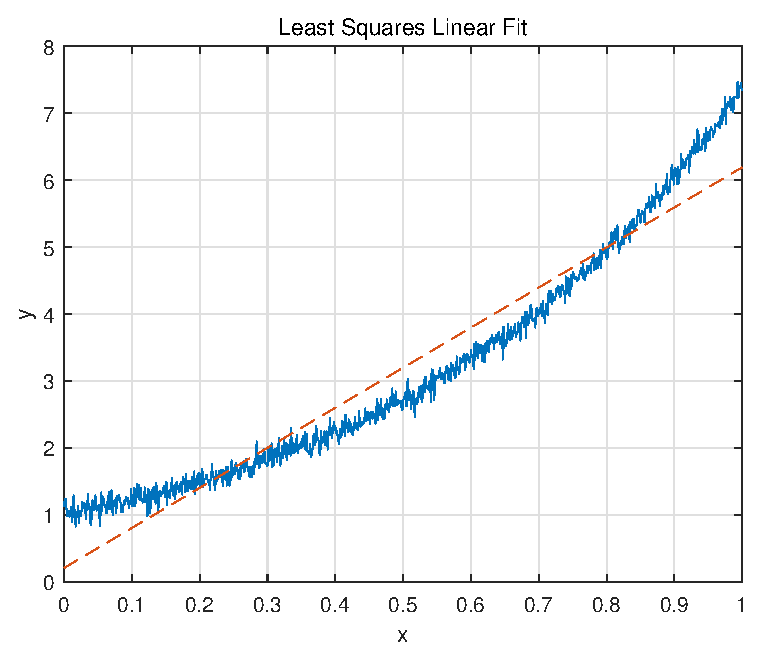
\includegraphics[scale=1]{Figure1.eps}
   \begin{center}Figure1: By setting the entries in vector x in the input data as the x coordinates and the entries in vector y as the y coordinates of the points of the line, and connect these points, the curvy line is obtained. Let A be the matrix formed with the first column being each entry of x with power 0, and the second column being each entry of x with power 1. Then use the least square method to compute the solution for the least square line with the normal equation $sol=inv(A^A)A^Ty$. The  $'--'$ line is obtained by setting the entries in vector x in the input data as the x coordinates and the entries of the linear combination $b=sol(1)x_1+sol(2)x_2$ as the y coordinates of the $'--'$ line.\end{center}\end{center}
(f)Given vectors x and y both with n entries as inputs which form a linear function $e+kx=y$ where $e$ and $k$ are constants, this program solves $e$ and $k$ by the least squares method by first creating a Vendermonde matrix A with the first column being each entry of x with power 0, and with the second column being each entry of x with power 1. Then by using the normal equation, the program computes the solution. The result is performed on Figure1 as the least square line $'--'$ over the plot of vectors x and y where the entries of x is on the horizontal axis and that of y is on the vertical axis.
\\\\\begin{large}Problem 2\end{large}
\\\\$null(A)={0}$ gives that Ax=0 only has the trivial solution. 
\\\\$\Rightarrow$ The vectors $\{a_1\, a_2\, ...\, a_n\}$ in a square matrix A with n$\times$n are linearly independent.
\\\\\begin{flushright}Hangshi Jin \\913142686\end{flushright}
$\Rightarrow$The dimension of span$\{a_1, a_2, ..., a_n\}$ is n.
\\\\$\Rightarrow$rank(A)$=$dim(range(A))$=$n$\Rightarrow$A has full rank.
\\\\$\Rightarrow$Since A is square and has full rank, it is invertible.\begin{flushright}\qed\end{flushright}
\begin{large}Problem 3\end{large}
\\\\Set $x=\begin{bmatrix}\cos\theta\\\sin\theta\end{bmatrix}\in R^2$ for $0\leq\theta\leq2\pi$, then $\lVert x\rVert_2=1$. 
\\\\Now we find, for $0\leq\theta\leq2\pi$\[\min\lVert x\rVert_1=\min\{|\cos\theta|+|\sin\theta|\}=1.\]
$\Rightarrow x=\begin{bmatrix}\cos\frac{a\pi}{2}\\\sin\frac{a\pi}{2}\end{bmatrix}$ achieves such minimum, where $a\in I$.
\\\\\begin{large}Problem 4\end{large}
\\\\By the definition of the induced matrix norm on $R^{m\times m}$,\[\lVert A\rVert\geq\frac{\lVert Ax_i\rVert}{\lVert x_i\rVert}\]\begin{flushright}for $1\leq i\leq m$.\end{flushright}
By the definition of eigenvalue, \[\frac{\lVert Ax_i\rVert}{\lVert x_i\rVert}=\frac{\lVert \lambda_i x_i\rVert}{\lVert x_i\rVert}=|\lambda_i|\frac{\lVert  x_i\rVert}{\lVert x_i\rVert}=|\lambda_i|,\]
$\Rightarrow$ \[\lVert A\rVert\geq\frac{\lVert Ax_i\rVert}{\lVert x_i\rVert}=|\lambda_i|.\]\begin{flushright}for $1\leq i\leq m$.\end{flushright}
Thus, we have\[\lVert A\rVert\geq\max_{1\leq i\leq m}|\lambda_i(A)|=\rho(A).\]
\begin{flushright}\qed\end{flushright}
\begin{large}Problem 5\end{large}
\[\lVert u\rVert_2\lVert v\rVert_2=\sqrt{u_1^2+\cdot\cdot\cdot+u_m^2}\cdot\sqrt{v_1^2+\cdot\cdot\cdot+v_n^2}=\sqrt{(u_1^2+\cdot\cdot\cdot+u_m^2)(v_1^2+\cdot\cdot\cdot+v_n^2)}\]
\[=\sqrt{u_1^2v_1^2+\cdot\cdot\cdot+u_1^2v_n^2+u_2^2v_n^2+\cdot\cdot\cdot+u_m^2v_n^2}=\sqrt{(u_1v_1)^2+\cdot\cdot\cdot(u_1v_n)^2+(u_2v_n)^2+\cdot\cdot\cdot+(u_mv_n)^2}\]
\[=\lVert uv^T\rVert_2=\lVert A\rVert_2\]\begin{flushright}\qed\end{flushright}
\begin{large}Problem 6\end{large}
\\\\(a)\[norm(A)=4.302775637731994\]
\begin{flushright}Hangshi Jin \\913142686\end{flushright}
(b)\[sqrt(max(eig(A'*A)))=4.302775637731995\]
\[\text{the relative error} = \frac{sqrt(max(eig(A'*A)))-norm(A)}{norm(A)}=2.064198774185416e^{-16}\approx0\]
(c)\[\lVert A\rVert_1=\max_{1\leq j\leq2}\sum_{i=1}^{3}|a_{ij}|=\sum_{i=1}^{3}|a_{i2}|=2+2+3=7\]
\[\lVert A\rVert_\infty=\max_{1\leq i\leq3}\sum_{j=1}^{2}|a_{ij}|=\sum_{j=1}^{2}|a_{3j}|=1+3=4\]
\[\lVert A\rVert_F=\sqrt{\sum_{i=1}^{3}\sum_{j=1}^{2}a_{ij}^2}=\sqrt{(1+4)+(0+4)+(1+9)}=\sqrt{19}\]
(d)\[\lVert x\rVert_1= 7.895242360521543\]
\[\lVert x\rVert_2=3.408079473961677\]
\[\lVert x\rVert_\infty=2.258846861003648\]
\[\lVert a\rVert_1=7.895048063565293\]
\[\lVert a\rVert_2=3.408079473961677\]
\[\lVert a\rVert_\infty=2.351901738628052\]
$\Rightarrow$\[\lVert x\rVert_2=\lVert a\rVert_2\]
(e)\[\lVert U\rVert_1=2.828427124746190\]
\[\lVert U\rVert_2=1.000000000000000\]
\[\lVert U\rVert_\infty=2.641845987495489\]
\[\lVert U\rVert_F=2.828427124746190\]
\begin{large}Problem 7\end{large}
\\\\(a)\[\begin{matrix}e+k=-1 &\text{for (1,-1),}\\e+2k=3&\text{for (2,3),}\\e+3k=1&\text{for (3,1).}\end{matrix}\]
$\Rightarrow$\[\begin{bmatrix}1&1\\1&2\\1&3\end{bmatrix}\begin{bmatrix}e\\k\end{bmatrix}=\begin{bmatrix}-1\\3\\1\end{bmatrix}\]
$\Rightarrow$\[\text{normal equation}=\begin{bmatrix}1&1&1\\1&2&3\end{bmatrix}\begin{bmatrix}1&1\\1&2\\1&3\end{bmatrix}\begin{bmatrix}e\\k\end{bmatrix}=\begin{bmatrix}1&1&1\\1&2&3\end{bmatrix}\begin{bmatrix}-1\\3\\1\end{bmatrix}\]
\\\\\begin{flushright}Hangshi Jin \\913142686\end{flushright}
(b)\[\begin{bmatrix}1&1&1\\1&2&3\end{bmatrix}\begin{bmatrix}1&1\\1&2\\1&3\end{bmatrix}\begin{bmatrix}e\\k\end{bmatrix}=\begin{bmatrix}1&1&1\\1&2&3\end{bmatrix}\begin{bmatrix}-1\\3\\1\end{bmatrix}\]
\[\begin{bmatrix}3&6\\6&14\end{bmatrix}\begin{bmatrix}e\\k\end{bmatrix}=\begin{bmatrix}3\\8\end{bmatrix}\]
\[x=\begin{bmatrix}e\\k\end{bmatrix}=\begin{bmatrix}-1\\1\end{bmatrix}\]
\end{document}